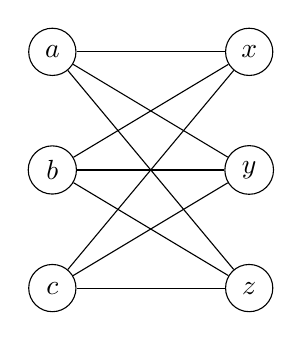
\begin{tikzpicture}

\node [circle, minimum height=0.6cm, draw] (v1) at (0,0) {$a$};
\node [circle, minimum height=0.6cm, draw] (v5) at (0,-1.5) {$b$};
\node [circle, minimum height=0.6cm, draw] (v6) at (0,-3) {$c$};
\node [circle, minimum height=0.6cm, draw] (v2) at (2.5,0) {$x$};
\node [circle, minimum height=0.6cm, draw] (v3) at (2.5,-1.5) {$y$};
\node [circle, minimum height=0.6cm, draw] (v4) at (2.5,-3) {$z$};
\draw  (v1) edge (v2);
\draw  (v1) edge (v3);
\draw  (v1) edge (v4);
\draw  (v5) edge (v2);
\draw  (v5) edge (v3);
\draw  (v5) edge (v4);
\draw  (v6) edge (v2);
\draw  (v6) edge (v3);
\draw  (v6) edge (v4);
\end{tikzpicture}